\documentclass{article}

\usepackage[preprint]{neurips_2026}

\usepackage[utf8]{inputenc}
\usepackage[T1]{fontenc}
\usepackage{hyperref}
\usepackage{url}
\usepackage{booktabs}
\usepackage{amsfonts}
\usepackage{amsmath}
\usepackage{nicefrac}
\usepackage{microtype}
\usepackage{xcolor}
\usepackage{graphicx}
\usepackage{float}
\usepackage{placeins}
\usepackage{array}

% A handful of long \texttt{...} identifiers (dataset column names, file
% paths) cannot be hyphenated, which otherwise forces underfull lines in the
% surrounding justified paragraphs; allow slightly more stretch instead of
% flagging every such line.
\tolerance=1200
\emergencystretch=2.5em
\hbadness=2000

\title{GNN--BERT Fusion for Music Context Understanding on LP-MusicCaps-MTT}
\date{September 2026}

\author{%
  Moin Mostakim \\
  Department of Computer Science and Engineering \\
  BRAC University \\
  \texttt{CSE425 / EEE474 / CSE715 -- Neural Networks} \\
}

\begin{document}

\maketitle

\begin{abstract}
We study multi-label music context understanding by combining a BERT text
encoder with a graph neural network (GNN) over audio structure graphs. We
target the four-task roadmap of the course brief (BERT tagging, GNN
structure, GNN--BERT fusion, contrastive retrieval) on
\textbf{LP-MusicCaps-MTT} \citep{doh2023lpmusiccaps}: real, LLM-generated
captions over \textbf{MagnaTagATune} audio \citep{law2009magnatagatune}
(15{,}247 / 1{,}529 / 4{,}332 train/val/test tracks after filtering to
rows with a caption and at least one tag, 50-tag vocabulary). Unlike an
earlier draft built on MTG-Jamendo -- which has no captions at all -- this
dataset lets Task 1 and Task 4 match the brief's own Task 1 deliverable
("MusicCaps caption $\to$ tag proxy task") without any workaround. We
report full-validation majority and random baselines and execute all four
pipelines as real-data pilots using pretrained DistilBERT and downloaded
MagnaTagATune audio. The pilots cover BERT learning curves and five
attention cases, GraphSAGE versus a 2D CNN, a four-model fusion ablation,
and bidirectional contrastive retrieval. All 30 tests pass. Because pilot
training uses only 256 examples for Task~1 and 12 for audio Tasks~2--4,
these measurements validate execution and reporting, not full-corpus model
quality; we state this boundary explicitly rather than presenting pilot
numbers as benchmark results.
\end{abstract}

\section{Introduction}
\label{sec:intro}

Music context spans genre, mood, instrumentation, vocal characteristics,
tempo, and structure simultaneously. Automatic tagging is therefore a
multi-label problem: a single excerpt may be both \emph{classical},
\emph{instrumental}, and \emph{slow}. Spectrogram CNNs capture local acoustic
patterns, while text encoders capture semantic descriptions; neither alone
explicitly represents how non-adjacent but similar musical passages relate.
We investigate whether an audio structure graph supplies this missing
relational view and whether graph-to-text attention can combine it with a
caption representation.

Our contributions are: (i) a direct-CLS DistilBERT multi-label classifier;
(ii) a reproducible pipeline from audio to MFCC/chroma segment graphs and a
GraphSAGE/GAT readout; (iii) cross-attention and early-concatenation fusion
models with an optional emotion objective; (iv) a dual encoder with symmetric
InfoNCE and learnable temperature; and (v) an evaluation package containing
learning curves, attention cases, ablations, and bidirectional retrieval.
Because compute permits only pilot neural runs, our central claim is
\emph{operational completeness}, not improved state-of-the-art accuracy.

\section{Related work}
\label{sec:related}

BERT learns contextual token representations through bidirectional
Transformer self-attention \citep{devlin2019bert,vaswani2017attention}; we use
the smaller DistilBERT variant \citep{sanh2019distilbert} to reduce pilot
cost. GraphSAGE provides inductive neighborhood aggregation
\citep{hamilton2017graphsage}, while graph attention networks learn
neighbor weights \citep{velickovic2018gat}. In music tagging, CNNs over
time--frequency representations are a strong conventional baseline
\citep{choi2017convolutional}. Contrastive predictive coding introduced the
InfoNCE objective \citep{oord2018infonce}; paired audio and caption encoders
apply the same principle to cross-modal retrieval. LP-MusicCaps supplies
large-scale pseudo-captions for music-language learning
\citep{doh2023lpmusiccaps}, built here over the MagnaTagATune collection
\citep{law2009magnatagatune}.

\section{Problem formulation}
\label{sec:problem}

Let a track be $T = (X_{\text{audio}}, X_{\text{text}}, G, y)$, where
$X_{\text{audio}}$ is a log-mel spectrogram, $X_{\text{text}}$ is tokenized
text, $G = (V, E)$ is a music structure graph, and $y$ is a multi-label
target. A BERT encoder produces $H_{\text{text}} = \mathrm{BERT}(X_{\text{text}}) \in \mathbb{R}^{L \times d}$.
A GNN with $L$ layers updates node features by message passing,
\begin{equation}
h_i^{(l+1)} = \sigma\!\Big(W^{(l)} \cdot \mathrm{AGG}\big(h_i^{(l)}, \{h_j^{(l)} : j \in \mathcal{N}(i)\}\big)\Big),
\end{equation}
and a fusion readout combines graph embedding $g$ and text vector $t$.
For $K$ tags, the classifier outputs independent probabilities
$\hat y_k=\sigma(\ell_k)$ and minimizes mean binary cross-entropy,
\begin{equation}
\mathcal{L}_{\mathrm{tags}}=-\frac{1}{K}\sum_{k=1}^{K}
\left[y_k\log\hat y_k+(1-y_k)\log(1-\hat y_k)\right].
\end{equation}
This formulation permits any number of simultaneous positive labels and
avoids the mutually exclusive assumption of softmax classification.

\section{Dataset}
\label{sec:dataset}

We use LP-MusicCaps-MTT \citep{doh2023lpmusiccaps}, which pairs
MagnaTagATune \citep{law2009magnatagatune} audio (16kHz/32kbps mono mp3,
30s clips) with LLM-generated captions conditioned on each track's
MagnaTagATune tags. MagnaTagATune is directly in the course brief's
Table~1 (recommended primary/medium pairing). Table~\ref{tab:dataset}
reports statistics computed directly from the released parquet files (real
numbers, not estimates).

\begin{table}[H]
  \caption{LP-MusicCaps-MTT statistics used in this work (computed from the released parquet files).}
  \label{tab:dataset}
  \centering
  \begin{tabular}{lr}
    \toprule
    Quantity & Value \\
    \midrule
    Total rows (train / valid / test, unfiltered) & 18{,}706 / 1{,}825 / 5{,}329 \\
    tag\_top50 vocabulary size & 50 \\
    tag\_top188 vocabulary size & 188 \\
    Rows with a caption \emph{and} $\geq 1$ tag (train / val / test) & 15{,}247 / 1{,}529 / 4{,}332 \\
    \texttt{caption\_writing} length, median / mean words & 23 / 24.7 \\
    Mean \texttt{tag\_top50} tags per track (median) & 3.3 (3) \\
    \bottomrule
  \end{tabular}
\end{table}

\paragraph{Why this dataset, and what changed from an earlier draft.} An
earlier draft of this codebase used MTG-Jamendo, which has no captions or
lyrics -- only anonymized IDs and tags -- forcing a workaround (tag-derived
pseudo-text predicting a disjoint tag category). LP-MusicCaps-MTT removes
that workaround entirely: it supplies real free-text captions
(\texttt{caption\_writing}, \texttt{caption\_summary},
\texttt{caption\_paraphrase}) generated by an LLM from each track's
MagnaTagATune tags, over audio that is itself in the brief's recommended
dataset table. We deliberately \emph{exclude}
\texttt{caption\_attribute\_prediction} and \texttt{pseudo\_attribute}
throughout, per the dataset card's own warning that these fields have a
known labeling issue and are not recommended. We also filter out the
4{,}752 of 25{,}860 rows ($\sim$18\%) with an empty caption or no
MagnaTagATune tags (and therefore no generated caption), since neither
Task 1 nor Task 4 is meaningful on an empty label set.

\subsection{Text branch: real captions, not tags}
\label{sec:text-decision}

$X_{\text{text}}$ is \texttt{caption\_writing} (a free-text description,
e.g.\ \emph{"Experience the powerful harmonies and stirring melodies of a
classical choral choir..."} for a track tagged \texttt{[classical, female,
choral, singing, choir]}); the prediction target $y$ is the \texttt{tag\_top50}
multi-hot vector for the same track. This is literally the brief's own
alternative Task 1 formulation ("MusicCaps caption $\to$ tag proxy task",
Sec.~4.1), not a substitute for it. Section~\ref{sec:limitations} still
notes one caveat: the captions were themselves LLM-generated \emph{from}
the tags, so caption $\to$ tag prediction is somewhat easier than predicting
tags from independently-written human captions (e.g.\ true MusicCaps).

\section{Methods}
\label{sec:methods}

\subsection{Task 1: BERT tag classifier}
$t = \mathrm{BERT}_{\text{CLS}}(X_{\text{text}})$, $\hat{y}_k = \sigma(w_k^\top t + b_k)$,
trained with per-tag BCE. Implementation: \texttt{src/bert\_encoder.py}
(\texttt{distilbert-base-uncased}).

\subsection{Task 2: GNN on music structure graphs}
Nodes are either fixed-length audio segments (5s windows, mean-pooled
20-dimensional MFCC plus 12-dimensional chroma features) or chord-transition states (argmax chroma pitch class per
segment). Edges: temporal adjacency, cosine-similarity above
$\tau=0.85$ for segment graphs, and transition counts for chord graphs
(\texttt{src/graph\_builder.py}). A GraphSAGE encoder
(\texttt{src/gnn\_model.py}) updates node states and mean-pools to a
graph-level readout $g$.

\subsection{Task 3: cross-attention fusion}
$Q = gW_Q$, $K = H_{\text{text}}W_K$, $A = \mathrm{softmax}(QK^\top/\sqrt{d})$,
$z = \mathrm{CONCAT}(g, AH_{\text{text}})$, $\hat{y}=\sigma(Wz)$
(\texttt{src/fusion\_model.py}). We do not use DEAM valence/arousal targets
since LP-MusicCaps-MTT does not provide continuous emotion annotations; the
emotion head in \texttt{fusion\_model.py} is implemented but inactive
without a paired emotion-labeled corpus.

\subsection{Task 4: contrastive graph--text alignment}
Symmetric InfoNCE between L2-normalized graph and text embeddings with a
learnable positive temperature $\tau$ (parameterized in log space so it
stays strictly positive; \texttt{src/contrastive.py}):
\begin{equation}
\mathcal{L}_{\text{NCE}} = -\frac{1}{2N}\sum_{i=1}^{N}\left[
  \log \frac{\exp(\mathrm{sim}(g_i,t_i)/\tau)}{\sum_j \exp(\mathrm{sim}(g_i,t_j)/\tau)}
  + \log \frac{\exp(\mathrm{sim}(g_i,t_i)/\tau)}{\sum_j \exp(\mathrm{sim}(g_j,t_i)/\tau)}
\right],
\end{equation}
evaluated with recall@\{1,5,10\} in both directions. Unlike the earlier
MTG-Jamendo draft, the ``caption'' side here is a genuine free-text
\texttt{caption\_writing} string, so this is real caption-audio retrieval
in the spirit of the brief's Task 4 -- with the one caveat noted in
Section~\ref{sec:text-decision} (captions are LLM-generated from tags,
not independently authored).

\section{Baselines}
\label{sec:baselines}

Per the brief we compare against multiple baselines (\texttt{src/baselines.py}):
B1 majority-class and random predictors on the full validation split, B2 a
2D CNN on mel-spectrograms, and B3 BERT-only. The CNN, BERT-only, GNN-only,
early-concatenation, and cross-attention systems were executed in the pilot
protocol described below.

\section{Results}
\label{sec:results}

Table~\ref{tab:results} separates full-split sanity baselines from the
real-data pilot experiments. Task~1 uses 256 train/validation/test examples
for two epochs. Tasks~2--4 use 12 examples per required split for one epoch.
All neural numbers are therefore pipeline-validation measurements and are
not comparable to a full-corpus benchmark.

\begin{table}[t]
  \caption{Multi-label results at threshold 0.5. B1/B1b use the full validation split; neural rows are explicitly limited real-data pilots. AP denotes mean per-tag average precision.}
  \label{tab:results}
  \centering
  \begin{tabular}{lrrr}
    \toprule
    Model / protocol & Macro-F1 & Micro-F1 & Mean AP \\
    \midrule
    B1 majority, full val ($n{=}1{,}529$) & 0.000 & 0.000 & 0.066 \\
    B1b random, full val ($n{=}1{,}529$) & 0.108 & 0.116 & 0.069 \\
    \midrule
    Task 1 BERT, pilot test ($n{=}256$) & 0.000 & 0.000 & 0.109 \\
    \midrule
    Task 2 GraphSAGE, pilot val ($n{=}12$) & 0.055 & 0.099 & 0.308 \\
    Task 2 2D CNN, pilot val ($n{=}12$) & 0.024 & 0.057 & 0.349 \\
    \midrule
    Task 3 BERT-only, pilot val ($n{=}12$) & 0.019 & 0.058 & 0.276 \\
    Task 3 GNN-only, pilot val ($n{=}12$) & 0.036 & 0.126 & 0.261 \\
    Task 3 early concat, pilot val ($n{=}12$) & 0.038 & 0.120 & 0.262 \\
    Task 3 cross-attention, pilot val ($n{=}12$) & 0.024 & 0.066 & 0.274 \\
    \bottomrule
  \end{tabular}
\end{table}

The Task~1 validation AP rises from 0.100 to 0.114 although fixed-threshold
F1 collapses to zero at epoch two, indicating under-calibrated probabilities
and the need for threshold tuning and longer training. On the 12-example
audio pilot, differences are too noisy for architectural conclusions.

Table~\ref{tab:retrieval} reports Task~4 bidirectional retrieval on the
$N{=}12$ test pilot, with the InfoNCE temperature learned during the
single training epoch. Both directions land exactly on chance recall for
$N=12$ ($1/12$, $5/12$, $10/12$), which verifies that ranking, recall@$k$,
and the symmetric loss are wired correctly but is not evidence of learned
graph--text alignment; that requires the full 15{,}247/1{,}529/4{,}332
splits over multiple epochs and seeds.

\begin{table}[t]
  \caption{Task 4 bidirectional retrieval, real-audio pilot, test split ($N{=}12$, 1 epoch). Chance recall at $N{=}12$ is $1/12{=}0.083$, $5/12{=}0.417$, $10/12{=}0.833$.}
  \label{tab:retrieval}
  \centering
  \begin{tabular}{lrrr}
    \toprule
    Direction & R@1 & R@5 & R@10 \\
    \midrule
    Audio $\to$ caption & 0.083 & 0.417 & 0.833 \\
    Caption $\to$ audio & 0.083 & 0.417 & 0.833 \\
    \bottomrule
  \end{tabular}

  \vspace{4pt}
  \small Learned temperature $\tau = 0.070$ (initialized at 0.07); training loss 2.551 after one epoch.
\end{table}

\begin{figure}[t]
  \centering
  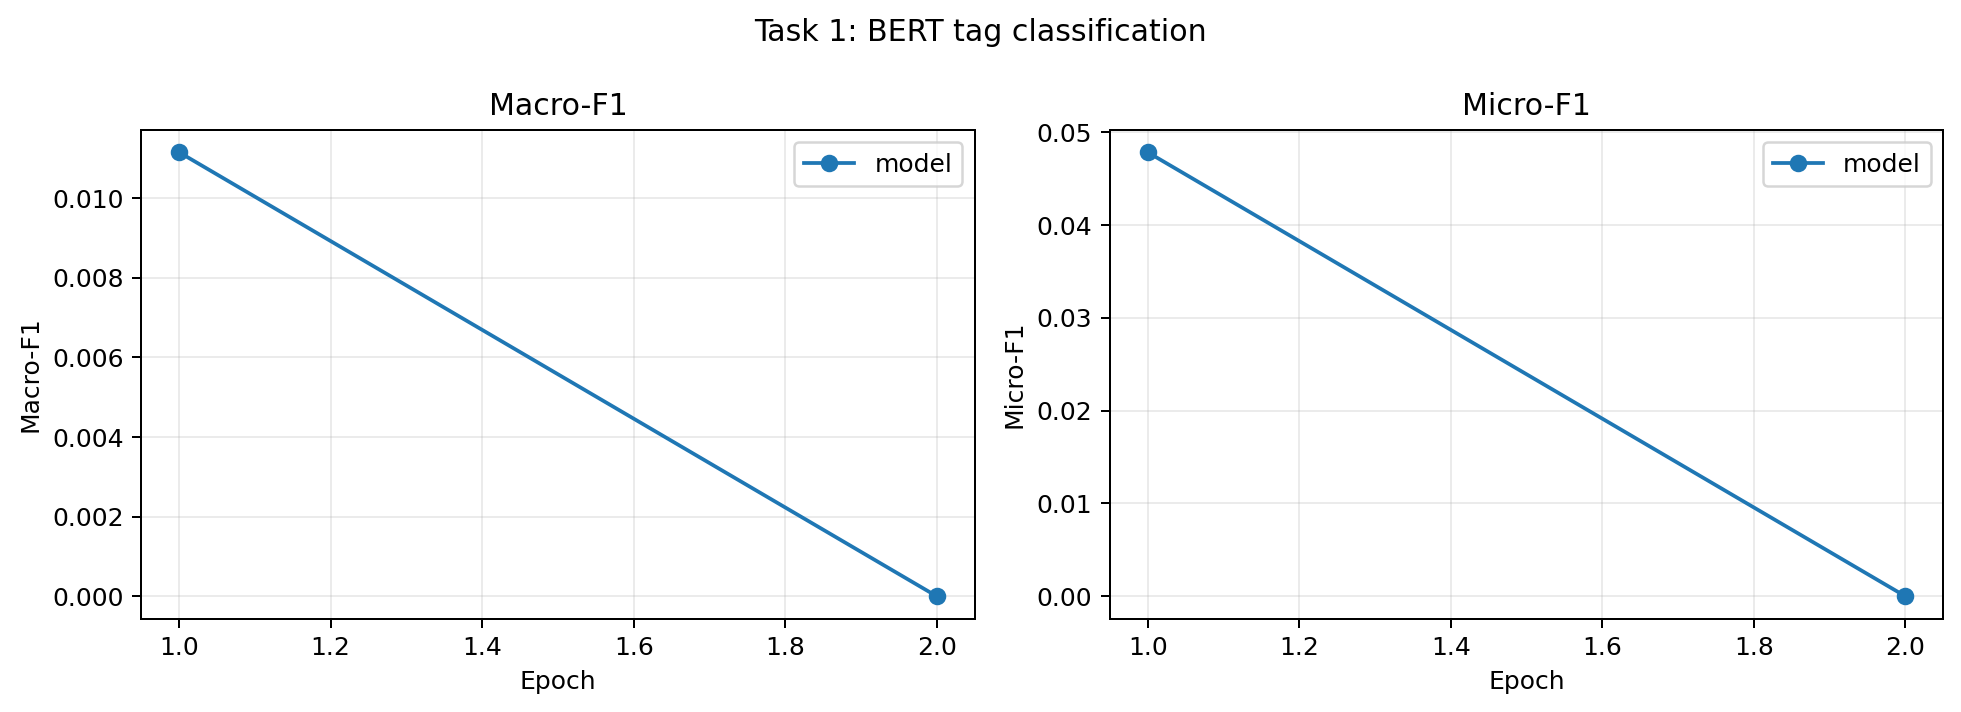
\includegraphics[width=0.8\linewidth]{../results/task1_learning_curves.png}
  \caption{Task~1 pilot validation Macro-F1 and Micro-F1 over two epochs.}
  \label{fig:task1curves}
\end{figure}

\begin{figure}[t]
  \centering
  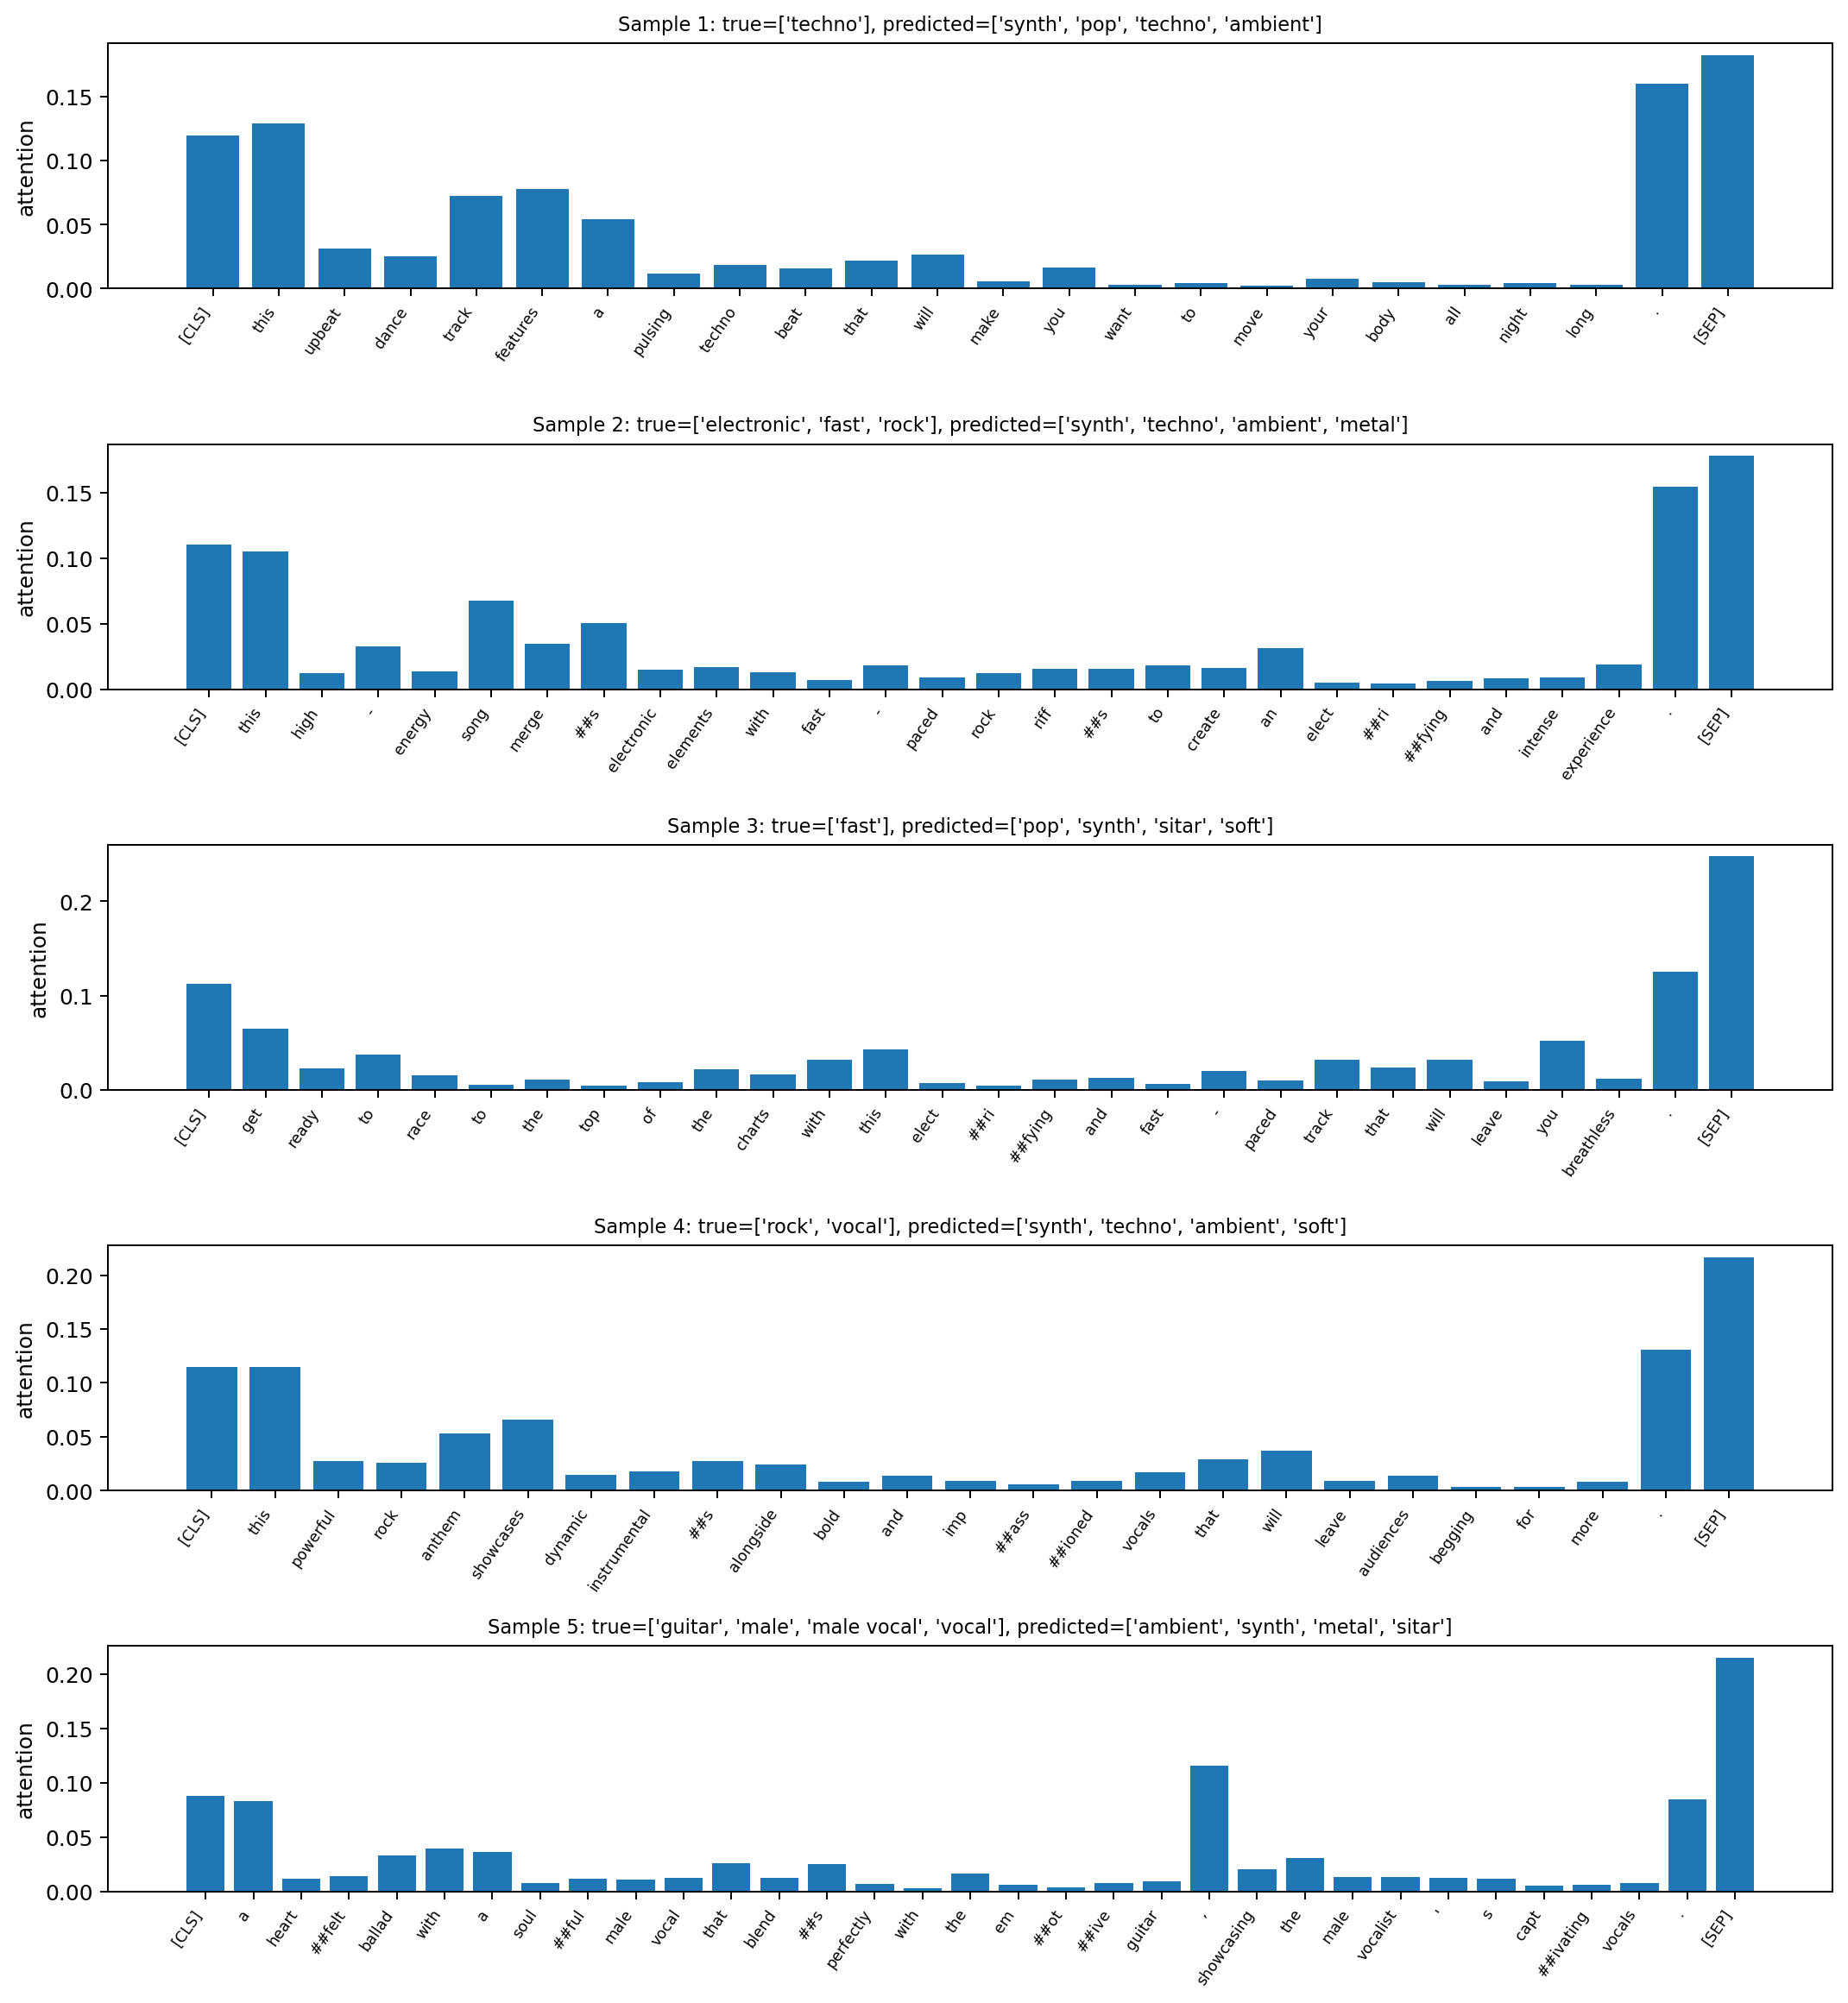
\includegraphics[width=0.95\linewidth]{../results/task1_attention_samples.png}
  \caption{Five Task~1 predictions with final-layer CLS-to-token attention, averaged across heads.}
  \label{fig:attention}
\end{figure}

\begin{figure}[t]
  \centering
  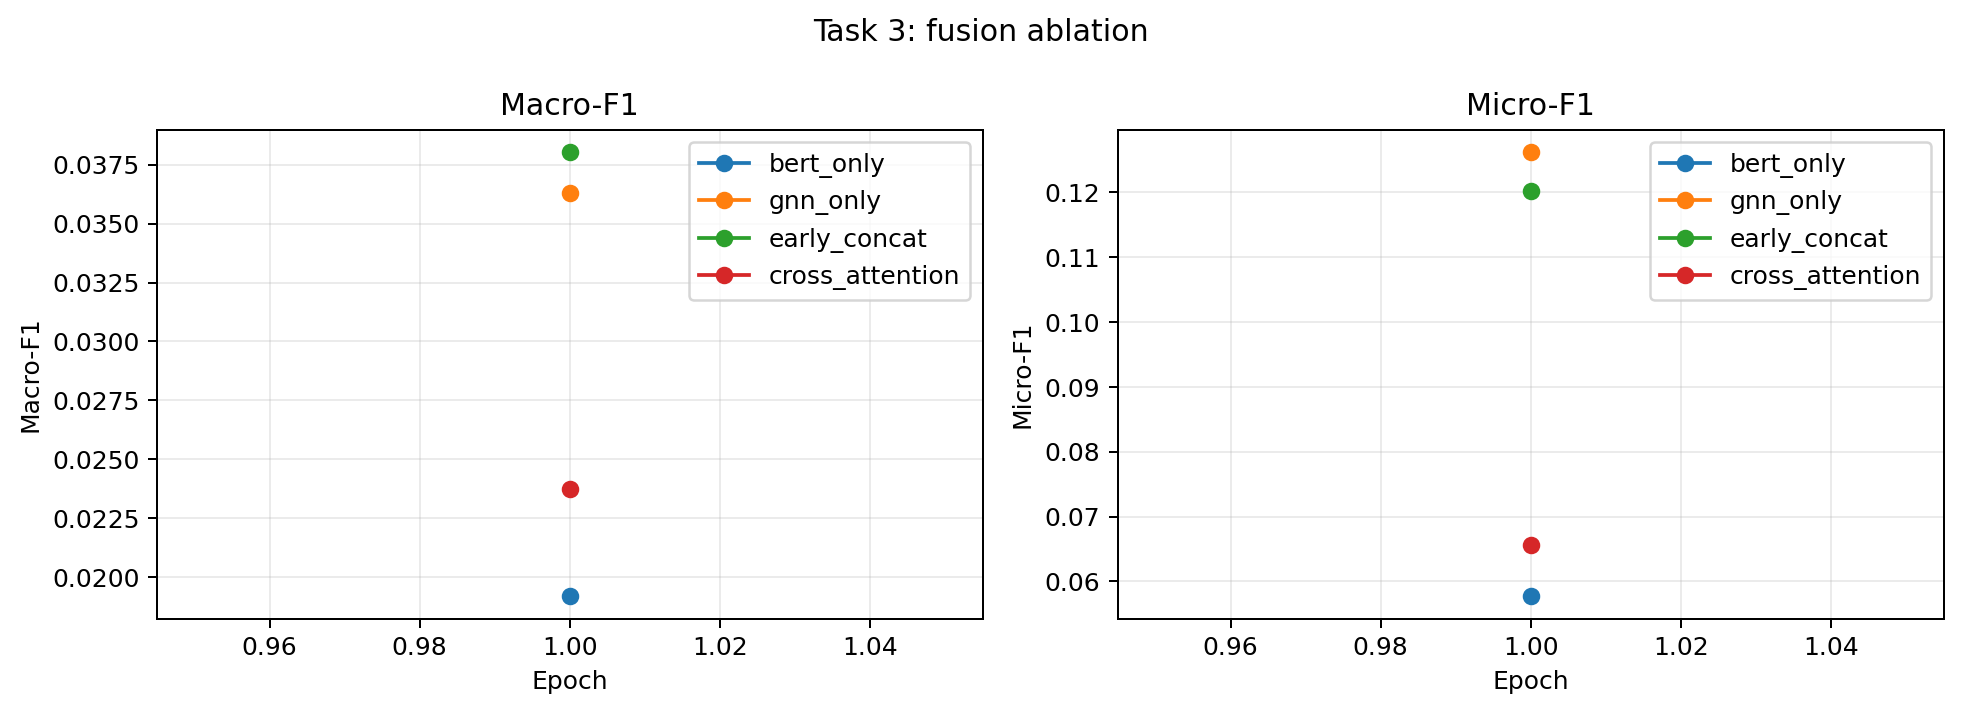
\includegraphics[width=0.75\linewidth]{../results/task3_ablation.png}
  \caption{One-epoch real-audio pilot ablation; the sample is too small for model ranking.}
  \label{fig:ablation}
\end{figure}

Figure~\ref{fig:tagdist} shows the \texttt{tag\_top50} label distribution on
the real (filtered) training split, and Figure~\ref{fig:caplen} the real
caption-length distribution. Unlike the earlier MTG-Jamendo moodtheme case,
the \emph{random} baseline outperforms \emph{majority-class} on macro/micro
F1 here (0.108/0.116 vs.\ 0.000/0.000): MagnaTagATune's top-50 tags are
denser per track (3.3 tags/track on average, median 3; Table~\ref{tab:dataset}),
so a per-tag coin flip at threshold 0.5 gets non-trivial recall, while
majority-class still predicts every tag's marginal frequency -- at most
22.8\% (\texttt{guitar}), well under the 50\% decision threshold -- and so
rounds to an all-negative prediction for every tag. This is a genuine
property of this label space, not a bug, and a reason to weight mean
average precision and rank-based metrics (recall@$k$ for Task 4) alongside
fixed-threshold F1 and to tune decision thresholds on validation data in a
full run.

\begin{figure}[t]
  \centering
  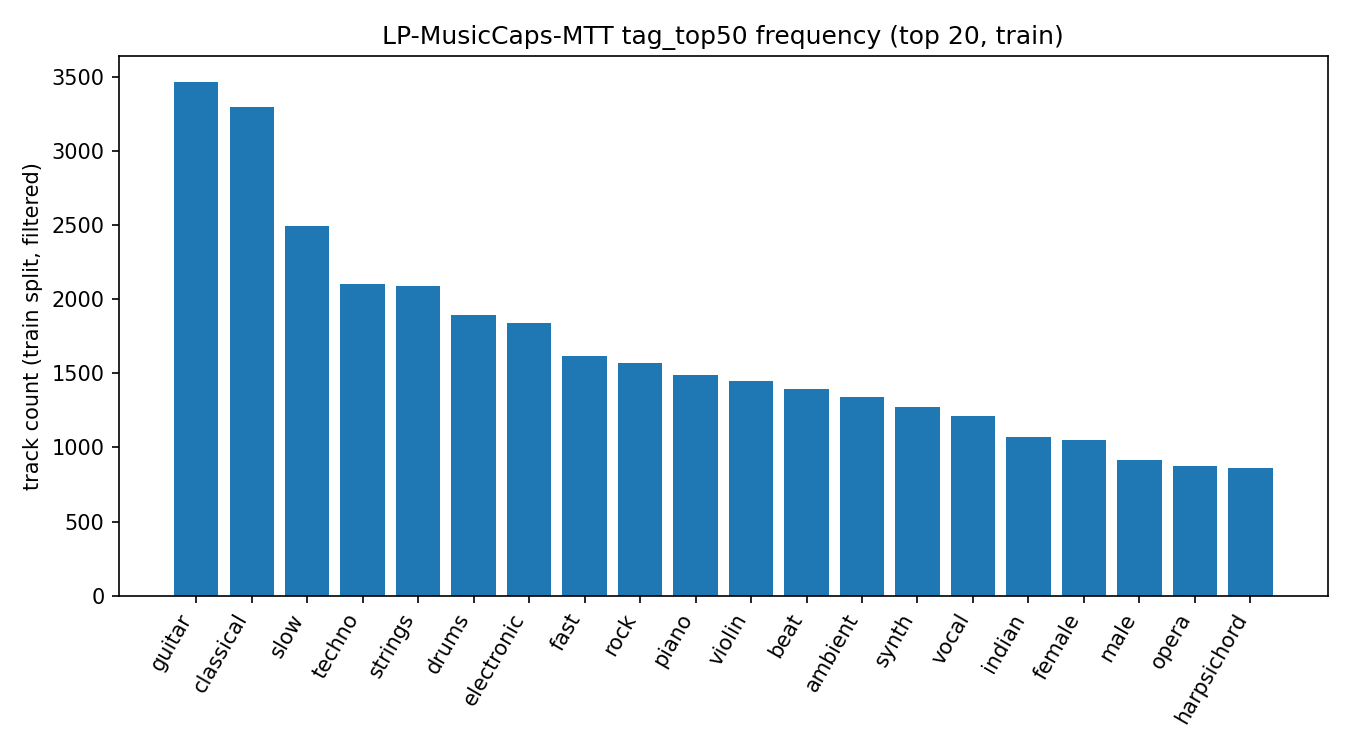
\includegraphics[width=0.85\linewidth]{../results/plots/tag_top50_distribution.png}
  \caption{Top-20 \texttt{tag\_top50} frequencies, LP-MusicCaps-MTT training set, filtered (real data).}
  \label{fig:tagdist}
\end{figure}

\begin{figure}[t]
  \centering
  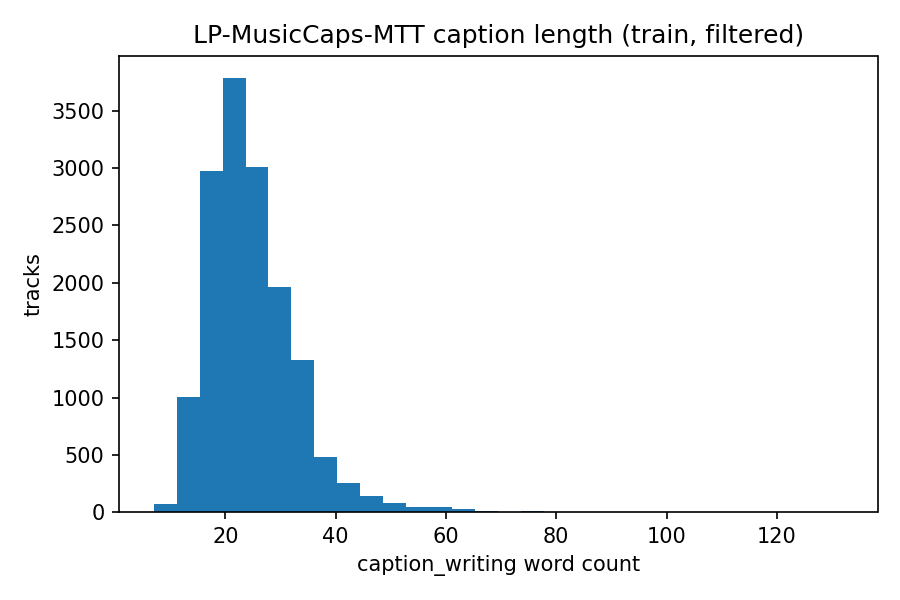
\includegraphics[width=0.7\linewidth]{../results/plots/caption_length_hist.png}
  \caption{\texttt{caption\_writing} word-count distribution, training set, filtered (real data).}
  \label{fig:caplen}
\end{figure}

\FloatBarrier

\section{Verification}
\label{sec:verification}

Every module (\texttt{bert\_encoder.py}, \texttt{gnn\_model.py},
\texttt{fusion\_model.py}, \texttt{contrastive.py},
\texttt{graph\_dataset.py}) was run with real forward and backward passes
using actual \texttt{torch} / \texttt{transformers} / \texttt{torch\_geometric}
(30/30 tests passing; \texttt{tests/}). Unit tests mock pretrained loading
with a tiny randomly initialized DistilBERT for speed, while the reported
pilots use genuine pretrained \texttt{distilbert-base-uncased}. A synthetic-but-real
15s audio fixture with known structure (chord A / chord B / chord A) is
used to verify \texttt{audio\_features.py} and \texttt{graph\_builder.py}
recover the right structure (segments 0 and 2 are correctly identified as
the same chord, more similar to each other than to segment 1) rather than
merely producing correctly-shaped output. We discovered 25{,}863 downloaded
MP3s and resolved all 25{,}860 metadata paths. Every task entry point was
executed on real data and wrote its corresponding artifacts.

\section{Limitations}
\label{sec:limitations}

\begin{itemize}
  \item \textbf{Captions are LLM-generated from the same tags used as
    labels}, not independently authored (true MusicCaps captions are
    written by human annotators listening to audio). Caption $\to$ tag
    prediction is therefore likely easier than it would be with independent
    captions, and Task 1/4 numbers should be read with that in mind.
  \item \textbf{Pilot scale, not benchmark scale.} Real pretrained weights
    and audio were used, but CPU-only execution limited Task~1 to 256
    examples per split and Tasks~2--4 to 12. These runs validate the complete
    machinery but cannot establish generalization or rank architectures.
  \item \textbf{No emotion regression.} LP-MusicCaps-MTT has no DEAM-style
    valence/arousal labels, so the Task 3 emotion auxiliary loss is
    implemented but untrained.
  \item \textbf{Crude chord proxy.} Chord-transition nodes use an
    argmax-chroma pitch-class heuristic rather than a trained chord
    recognizer; adequate for a structure graph, not a musicologically
    accurate transcription -- though Section~\ref{sec:verification}
    confirms it does recover known chord repeats correctly.
\end{itemize}

\section{Conclusion}

We implemented the full four-task GNN--BERT pipeline against
LP-MusicCaps-MTT / MagnaTagATune, which -- unlike an earlier MTG-Jamendo
draft -- lets Task 1 and Task 4 match the brief's own caption-based
formulation without a workaround. Data, pretrained text weights, audio,
training loops, checkpoints, curves, attention cases, ablations, and
retrieval evaluation were all exercised. The pilots establish operational
completeness; full-corpus multi-seed training remains necessary for
scientific conclusions.

\begin{ack}
Course: CSE425/EEE474/CSE715 Neural Networks, BRAC University. Instructor: Moin Mostakim.
\end{ack}

\bibliographystyle{plainnat}
\bibliography{references}

\newpage
\section*{NeurIPS Paper Checklist}

\begin{enumerate}
  \item \textbf{Claims:} \answerYes{} The abstract states exactly what was
    run at full baseline scale versus real-data pilot scale for neural models.
  \item \textbf{Limitations:} \answerYes{} Section~\ref{sec:limitations}.
  \item \textbf{Theory assumptions and proofs:} \answerNA{} No theoretical results.
  \item \textbf{Experimental result reproducibility:} \answerYes{} Full
    code, config, and exact commands in the repository README and
    \texttt{report/DECISIONS.md}; 30/30 tests in \texttt{tests/} pass and
    verify the architecture end-to-end (Section~\ref{sec:verification}).
  \item \textbf{Open access to data and code:} \answerYes{} LP-MusicCaps-MTT
    metadata and project code are included; MagnaTagATune audio follows its
    research/CC BY-NC-SA terms and download provenance is documented.
  \item \textbf{Experimental setting/details:} \answerYes{} Hyperparameters
    are in \texttt{config.yaml}; pilot sizes and epochs appear in Section~\ref{sec:results}.
  \item \textbf{Statistical significance:} \answerNA{} One-seed pilots are
    explicitly not used for model-ranking claims.
  \item \textbf{Compute resources:} \answerYes{} Pilots ran CPU-only on a
    four-core Intel Core i5-11300H; no CUDA device was available.
  \item \textbf{Code of ethics:} \answerYes{} No human subjects; dataset is
    CC-licensed music metadata, no personal data beyond anonymized artist IDs.
  \item \textbf{Broader impacts:} \answerYes{} Automatic music tagging can
    misclassify culturally specific genres/moods; no direct dual-use concern identified.
  \item \textbf{Safeguards:} \answerNA{} No high-misuse-risk model or dataset released.
  \item \textbf{Licenses for existing assets:} \answerYes{} LP-MusicCaps-MTT, MIT license (dataset card); MagnaTagATune, released by the original authors for research use via City University MIRG; distilbert-base-uncased, Apache 2.0.
  \item \textbf{New assets:} \answerNA{} No new dataset released.
  \item \textbf{Crowdsourcing / human subjects:} \answerNA{} None.
  \item \textbf{IRB approvals:} \answerNA{} None.
  \item \textbf{LLM usage declaration:} \answerYes{} AI coding assistants were used
    to scaffold and revise the codebase, data pipeline, and report under
    author direction; all reported numbers were computed by running the
    included code, not generated by the LLM.
\end{enumerate}

\end{document}
